%% LyX 2.3.6.1 created this file.  For more info, see http://www.lyx.org/.
%% Do not edit unless you really know what you are doing.
\documentclass[english]{article}
\usepackage[T1]{fontenc}
\usepackage[latin9]{inputenc}
\usepackage{geometry}
\geometry{verbose,tmargin=2.5cm,bmargin=2.5cm,lmargin=2.5cm,rmargin=2.5cm}
\usepackage{textcomp}
\usepackage{graphicx}

\makeatletter

%%%%%%%%%%%%%%%%%%%%%%%%%%%%%% LyX specific LaTeX commands.
%% Because html converters don't know tabularnewline
\providecommand{\tabularnewline}{\\}

\makeatother

\usepackage{babel}
\begin{document}
{[}SPLIT\_HERE{]}
\begin{enumerate}
\item \textbf{{[}HCI/PRELIM/9597/2019/P1/Q1{]} }

The manager of a private carpark wants to process the daily data of
people using the carpark. The carpark is open from 8am to 11pm and
the carpark charge is as follows:
\begin{itemize}
\item Before 5pm: \$1.50 per hour or part thereof 
\item After 5pm, \$3.00 per entry regardless of the duration
\end{itemize}
However, if a car enters before 5pm and leaves after 5pm, the charge
involves both rules. For example, if the car stays in the carpark
from 2.45pm to 6.30pm, it is broken down to 2 hours 15 minutes before
5pm and 1 hour 30 minutes after 5pm. Hence the charge will be \$1.50
{*} 3 + \$3.00 = \$7.50. 

Each day the carpark electronic system generates a file\texttt{ CARPARK.txt}.
Each record in the file has the following format:
\noindent \begin{center}
\texttt{<CARPLATE NUMBER>,<START TIME>,<END TIME>}
\par\end{center}

For example, \texttt{SLX2315A,0940,1415} means that a car with car
plate number SLX2315A entered the carpark at 9.40am and left at 2.15pm. 

You are \textbf{not} allowed to use any built-in functions for time
processing. 

\subsection*{Task 1.1 }

Write program code for the \texttt{Price} function using the following
specification:
\noindent \begin{center}
\texttt{FUNCTION Price (start: STRING, end: STRING) : FLOAT}
\par\end{center}

The function has two string parameters \texttt{start}, \texttt{end}
which refers to the start and end time when the car parked. The function
returns the carpark charge as a float. 

\subsection*{Evidence 1 }

Your program code.\hfill{} {[}5{]}

\subsection*{Task 1.2 }

Write a program code to perform the following task for the manager:
\begin{itemize}
\item Read data from \texttt{CARPARK.txt }
\item Write all the car plate numbers and corresponding carpark charges
to another file \texttt{CHARGE.txt}, in the following format: 
\noindent \begin{center}
\texttt{<CARPLATE NUMBER>,<CARPARK CHARGE>}
\par\end{center}

\noindent \begin{center}
\texttt{<CARPLATE NUMBER>,<CARPARK CHARGE>}
\par\end{center}
\item Output the total charges for the day
\end{itemize}

\subsection*{Evidence 2 }

Your program code.\hfill{} {[}7{]}

\subsection*{Evidence 3}

One screenshot showing the program output and contents of \texttt{CHARGE.txt}
from running the program.\hfill{} {[}3{]}

{[}SPLIT\_HERE{]}
\item \textbf{{[}HCI/PRELIM/9597/2019/P1/Q2{]} }

When a list of integers has repeated numbers, the searching and sorting
algorithms can be different. The task is to perform an insertion sort
before a binary search is executed. 

\subsection*{Task 2.1 }

Write the program code for a procedure to implement insertion sort
in ascending order. The input parameter is a list of integers which
may have repeated numbers. 

\subsection*{Evidence 4}

Your program code.\hfill{} {[}4{]}

\subsection*{Task 2.2 }

Write the program code for a procedure to implement binary search
for a targeted integer. The input parameter is an ordered list of
integers which may have repeated numbers. The procedure outputs all
the indices at which the target appears, or \texttt{\textminus 1}
if the target is not found. 

\subsection*{Evidence 5 }

Your program code. \hfill{}{[}9{]}

\subsection*{Task 2.3 }

The file \texttt{NUMBERS.txt} contains one integer at each line. Write
a program that uses the procedures in previous tasks and performs
the following task: 
\begin{itemize}
\item Reads the text file \texttt{NUMBERS.txt}, 
\item Perform insertion sort, and outputs the list of integers in a row, 
\item Prompts the user to provide a target to be searched, 
\item Perform a binary search and output an appropriate message
\end{itemize}

\subsection*{Evidence 6 }

Your program code.\hfill{} {[}4{]}

\subsection*{Task 2.4 }

Draw up \textbf{three} suitable tests and provide screenshot evidence
for your testing. 

\subsection*{Evidence 7 }

Annotated screenshots for each test data run. \hfill{}{[}3{]}

{[}SPLIT\_HERE{]}
\item \textbf{{[}HCI/PRELIM/9597/2019/P1/Q3{]} }

The examinations department of a school needs to keep long-term records
of the overall examination achievements of its students.

Students at the school have two main choices. Firstly, they can take
a variety of subjects and achieve an Academic Diploma. A diploma gives
them the opportunity to go to university. Secondly they can achieve
a Skills Certificate where they focus on one particular area (such
as IT). This gives them the necessary skills to start a career in
their chosen area.

The examinations department decides to store the following data:
\begin{itemize}
\item \texttt{StudID} is used to uniquely identify a particular student
and is six digits. The first four digits represent the year that the
student started at the school and the last two digits are used to
make the \texttt{StudID} unique e.g. 201804.
\item \texttt{Name} is the name of the student and is at most 30 characters.
\item \texttt{StudType} is the type of student and can have the values \textquoteleft D\textquoteright{}
or \textquoteleft S\textquoteright .
\item \texttt{SkillArea} is text and gives the area that the student acquired
skills in. It can have one of three values: \textquoteleft IT\textquoteright ,
\textquoteleft Business\textquoteright{} or \textquoteleft Accountancy\textquoteright .
\item \texttt{NoOfSub} is the number of subjects studied by those taking
the Diploma. 
\item \texttt{Result} is a single character and is used to indicate the
overall grade awarded. For those students who took the Skills Certificate
the grades could be Distinction (D), Merit (M), Pass (P) or Fail (F).
For those who took the Diploma the grade could be one of the letters
A to F. Grade A to E are passes. Grade F is a fail.
\end{itemize}
The program design for a solution to this problem is to be implemented
with object-oriented programming with the following three classes:
\begin{center}
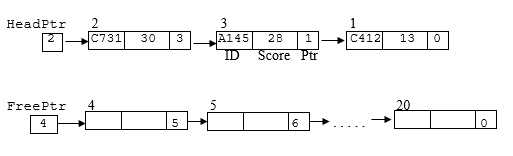
\includegraphics[width=0.5\paperwidth]{C:/Users/Admin/Desktop/Github/question_bank/LyX/static/img/9597-HCI-2019-P1-Q4-1}
\par\end{center}

\subsection*{Task 3.1 }

Write program code to define the classes \texttt{Student}, \texttt{Diploma}
and \texttt{SkillsCert}.

\subsection*{Evidence 8}

Program code for the three classes in Task 3.1. \hfill{}{[}6{]}

Assume that a file, \texttt{STUDENT.txt}, which contains details of
each student, has been created for you. The format of each student
record is as follows: 
\noindent \begin{center}
\texttt{<StudID>|<Name>|<StudType>|<SkillArea>|<NoOfSub>|<Result>}
\par\end{center}
\begin{itemize}
\item \texttt{SkillArea} would have the value \textquoteleft Diploma\textquoteright{}
if the student is taking a Diploma. 
\item \texttt{NoOfSub} would have the value 0 for those taking the Skills
Certificate.
\item \texttt{Result} is left blank initially. 
\end{itemize}

\subsection*{Task 3.2 }

Write a module, \texttt{ENTER\_RESULT}, which, when called, will ask
the user for a particular \texttt{StudID} whose result is to be entered.
Using the student ID that has been input, the corresponding student
record will be located in \texttt{STUDENT.txt}. The student data will
be displayed to the user. The user will be allowed to enter the result
for the student. The amended record will be stored back in \texttt{STUDENT.txt}. 

The student ID and result that have been input should be validated. 

If the \texttt{StudID} does not exist, the user will be given an appropriate
message.

\textbf{You are expected to make use of the classes you designed in
Task 3.1}.

Run the program \textbf{three} times. Use the following data input,
and produce a screenshot for each. 
\noindent \begin{center}
\begin{tabular}{cc}
StudID & Result\tabularnewline
\hline 
\texttt{201701} & \texttt{A}\tabularnewline
\texttt{201801} & \texttt{B}\tabularnewline
\texttt{201901} & \texttt{M}\tabularnewline
\end{tabular}
\par\end{center}

\subsection*{Evidence 9}

Program code for Task 3.2 \hfill{}{[}8{]}

\subsection*{Evidence 10 }

Three screenshots showing the test runs and final contents of \texttt{STUDENT.txt}
to show evidence that successful updates have been carried out. \hfill{}{[}2{]}

\subsection*{Task 3.3}

Implement code as specified below.

A report should be generated and displayed which will list the students
whose result has still not been entered into the \texttt{STUDENT.txt}
file. The report will list, for each different starting year: 
\begin{itemize}
\item \texttt{StudID} 
\item \texttt{Name} 
\item \texttt{StudType}
\item \texttt{SkillArea} or \texttt{NoOfSub} depending upon the value of
\texttt{StudType} 
\end{itemize}
In addition the number of each student type for each year will also
be output.

A sample output is shown below.
\noindent \begin{center}
\begin{tabular}{llll}
Year: 2017 &  &  & \tabularnewline
\hline 
\texttt{201715} & FLoo & D & 6\tabularnewline
\texttt{201708} & BLang & D & 5\tabularnewline
\texttt{201710} & LArms & S & IT\tabularnewline
Diplomas: & 2 &  & \tabularnewline
Skills: & 1 &  & \tabularnewline
\end{tabular}
\par\end{center}

\noindent \begin{center}
\begin{tabular}{llll}
Year: 2018 &  &  & \tabularnewline
\hline 
\texttt{201813} & FJean & D & 7\tabularnewline
\texttt{201817} & ABright & D & 7\tabularnewline
Diplomas: & 2 &  & \tabularnewline
Skills: & 0 &  & \tabularnewline
\end{tabular}
\par\end{center}

\noindent \begin{center}
\begin{tabular}{llll}
Year: 2019 &  &  & \tabularnewline
\hline 
\texttt{201905} & Alfie & S & Business\tabularnewline
\texttt{201903} & GKoh & D & 8\tabularnewline
Diplomas: & 1 &  & \tabularnewline
Skills: & 1 &  & \tabularnewline
\end{tabular}
\par\end{center}

\subsection*{Evidence 11 }

Program code for Task 3.3. \hfill{}{[}8{]}

\subsection*{Evidence 12 }

Screenshot of the output produced.\hfill{} {[}2{]}

{[}SPLIT\_HERE{]}
\item \textbf{{[}HCI/PRELIM/9597/2019/P1/Q4{]} }

A game maintains the player IDs and their scores in an ordered linked
list. The player with the highest score is stored at the first node
while the player with the lowest score is stored at the last node. 

The program to implement the linked list abstract data type will use
two classes, \texttt{ListNode} and \texttt{LinkedList}. 

The \texttt{ListNode} class has the following properties:
\noindent \begin{center}
\begin{tabular}{|l|l|l|}
\hline 
\texttt{\hspace{0.01\columnwidth}}Identifier & \texttt{\hspace{0.01\columnwidth}}Data Type & \texttt{\hspace{0.05\columnwidth}}Description\tabularnewline
\hline 
\texttt{ID} & \texttt{STRING} & The ID of the player. All IDs are unique and have the format \texttt{L999}
where \texttt{L} is any uppercase letter and \texttt{9} is a digit.\tabularnewline
\hline 
\texttt{Score} & \texttt{INTEGER} & The score of the player.\tabularnewline
\hline 
\texttt{Ptr} & \texttt{INTEGER} & The pointer to the next node.\tabularnewline
\hline 
\end{tabular}
\par\end{center}

The \texttt{LinkedList} class has the following properties: 
\noindent \begin{center}
\begin{tabular}{|l|l|l|}
\hline 
\texttt{\hspace{0.01\columnwidth}}Identifier & \texttt{\hspace{0.01\columnwidth}}Data Type & \texttt{\hspace{0.05\columnwidth}}Description\tabularnewline
\hline 
\texttt{Node} & \texttt{ARRAY{[}1..20{]} OF ListNode} & 1-D array stores the nodes that make the ordered linked list. The
unused nodes are linked together into a free list.\tabularnewline
\hline 
\texttt{HeadPtr} & \texttt{INTEGER} & Pointer to the first node in the ordered list.\tabularnewline
\hline 
\texttt{FreePtr} & \texttt{INTEGER} & Pointer to the first node in the free list.\tabularnewline
\hline 
\end{tabular}
\par\end{center}

The following diagram shows an example of a linked list object. This
example list consists of three nodes, linked in descending order of
the game scores. The unused nodes are linked to form a free list.
\begin{center}
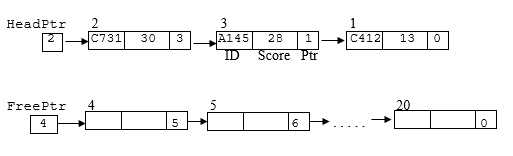
\includegraphics[width=0.5\paperwidth]{C:/Users/Admin/Desktop/Github/question_bank/LyX/static/img/9597-HCI-2019-P1-Q4-1}
\par\end{center}

\subsection*{Task 4.1}

Write program code for the classes \texttt{ListNode} and \texttt{Linkedlist}
to declare all the required variables and create the initial empty
linked list which contains all 20 nodes.

Add statement(s) to initialise the empty ordered linked list.

\subsection*{Evidence 13 }

Your program code for Task 4.1. \hfill{}{[}6{]}

\subsection*{Task 4.2 }

Write code to implement a method \texttt{AddInOrder} that will add
a new node with player\textquoteright s ID and score into the ordered
linked list in descending order of the scores. Node added to the ordered
linked list should be taken from the free list. 

Assume that all players have different scores.

\subsection*{Evidence 14 }

Your program code for Task 4.2.\hfill{} {[}7{]}

\subsection*{Task 4.3 }

Write a procedure \texttt{OutputData} which displays the value of
\texttt{HeadPtr}, the value of \texttt{FreePtr} and the contents of
\texttt{Node} array in index order.

\subsection*{Evidence 15 }

Your program code for Task 4.3.\hfill{} {[}3{]}

The files \texttt{SCORES1.txt} and \texttt{SCORES2.txt} contain the
game data. Each entry has the following format: \texttt{<Player ID>,<Score>} 

\subsection*{Task 4.4 }

Write a main program to:
\begin{itemize}
\item Create a linked list object 
\item Read all player data from \texttt{SCORES1.txt} and add them to the
linked list by calling procedure \texttt{AddInOrder}. 
\item Your program will then call procedure \texttt{OutputData}.
\end{itemize}

\subsection*{Evidence 16 }

Screenshot showing the output from running the program in Task 4.4
using \texttt{SCORES1.txt} file. \hfill{}{[}2{]}

\subsection*{Task 4.5 }

Amend your \texttt{AddInOrder} program code in Task 4.2 so that if
two or more players have the same score, they are stored in alphabetical
player ID order. Use the file \texttt{SCORES2.txt} to test your program
code.

The following diagram shows an example of an ordered linked list where
players \texttt{C412} and \texttt{B321} have the same game score of
\texttt{13} points. 
\begin{center}
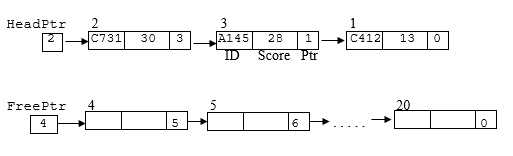
\includegraphics[width=0.5\paperwidth]{C:/Users/Admin/Desktop/Github/question_bank/LyX/static/img/9597-HCI-2019-P1-Q4-1}
\par\end{center}

\subsection*{Evidence 17 }

The amended program code for method \texttt{AddInOrder}. \hfill{}{[}4{]}

\subsection*{Evidence 18}

Screenshot showing the output from running the program in Task 4.4
using \texttt{SCORES2.txt} file. \hfill{}{[}2{]}

\subsection*{Task 4.6 }

A method \texttt{DisplayByRank} is to be added, which outputs all
player IDs and their scores stored in the ordered linked list in rank
order. If multiple players record the same score, they will have the
same rank. 

Below is a sample of screen output:
\noindent \begin{center}
\begin{tabular}{lll}
\texttt{Rank} & \texttt{Player ID} & \texttt{Score}\tabularnewline
\texttt{1} & \texttt{F111} & \texttt{45}\tabularnewline
\texttt{1} & \texttt{G333} & \texttt{45}\tabularnewline
\texttt{1} & \texttt{Z333} & \texttt{45}\tabularnewline
\texttt{4} & \texttt{C333} & \texttt{38}\tabularnewline
\texttt{5} & \texttt{B111} & \texttt{25}\tabularnewline
\texttt{5} & \texttt{Q333} & \texttt{25}\tabularnewline
\texttt{7} & \texttt{E333} & \texttt{12}\tabularnewline
\end{tabular}
\par\end{center}

Write program code to:
\begin{itemize}
\item Implement this method 
\item Test the program code with the data from Task 4.5.
\end{itemize}

\subsection*{Evidence 19 }

Program code for Task 4.6. \hfill{}{[}7{]}

\subsection*{Evidence 20}

Screenshot of the program output.\hfill{} {[}2{]}

\subsection*{Task 4.7 }

Write a recursive \texttt{ReverseTraversal} procedure that will traverse
the linked list in reverse order and output players\textquoteright{}
IDs and scores in ascending scores order.

Include a call to the procedure from your main program.

Test the program code with the data from Task 4.5.

\subsection*{Evidence 21 }

Your program code for Task 4.7.\hfill{}{[}4{]}

\subsection*{Evidence 22}

Screenshot showing the program execution to test the \texttt{ReverseTraversal}
method. \hfill{}{[}2{]}

{[}SPLIT\_HERE{]}
\item \textbf{{[}HCI/PRELIM/9597/2019/P2/Q1{]} }

A bookshop wishes to expand its business from a brick and mortar shop
to allow for online sales. A software company has been engaged by
the bookshop to develop the online sales system. 
\begin{enumerate}
\item The analyst decides to adopt a top-down approach to the design. What
are the advantages of using top-down design to solve complex problems?\hfill{}
{[}3{]} 
\end{enumerate}
The project manager decides to use some project management tool in
the planning of the project. Below is the list of activities along
with their required time for completion.
\noindent \begin{center}
\begin{tabular}{|c|c|c|}
\hline 
Activity & Expected completion time (day) & Preceded by\tabularnewline
\hline 
\hline 
A & 2 & -\tabularnewline
\hline 
B & 3 & A\tabularnewline
\hline 
C & 1 & B\tabularnewline
\hline 
D & 3 & B\tabularnewline
\hline 
E & 4 & C\tabularnewline
\hline 
F & 3 & D\tabularnewline
\hline 
G & 2 & A\tabularnewline
\hline 
H & 5 & G\tabularnewline
\hline 
I & 3 & E, F, H\tabularnewline
\hline 
\end{tabular}
\par\end{center}
\begin{enumerate}
\item[(b)]  Construct the PERT chart for the activities, indicating the earliest
start time and latest start time of each activity. \hfill{}{[}3{]}
\item[(c)]  Which tasks are on the critical path of the Program Evaluation and
Review Technique (PERT) chart? \hfill{}{[}1{]}
\item[(d)]  What is the slack time for Task C and G? \hfill{}{[}2{]}
\item[(e)]  The person working on Task C tells the project manager he cannot
start work until one day after the scheduled starting date. What impact
would this have on the completion date of the project? Why?\hfill{}
{[}2{]}
\item[(f)]  Task A will be delayed by 2 days for some reason. If the project
manager still wants to finish the project within the original time
frame, he will need to shorten the time for one or more of the tasks.
What steps can he take to reduce the number of days allocated to a
task? \hfill{}{[}2{]}
\item[(g)]  The project manager decides to reduce the time needed for Tasks
D and F by one day each. How effective will this reduction be in achieving
his aim of maintaining the original finish time for the project? What
can he do for it to be more effective?\hfill{} {[}2{]}
\item[(h)]  Produce a Gantt chart based on the above information. \hfill{}{[}2{]}
\item[(i)]  Give \textbf{one} reason why a Gantt chart may be preferred over
a PERT chart.\hfill{} {[}1{]}
\end{enumerate}
{[}SPLIT\_HERE{]}
\item \textbf{{[}HCI/PRELIM/9597/2019/P2/Q2{]} }

Customers can view a catalogue of books and order from its website.
Payment is made by the customer forwarding their credit card details,
which are processed immediately. Details of the orders are matched
against the stock file to check for availability of items before packing
lists are produced and sent to the packing department.
\begin{enumerate}
\item Draw a data flow diagram to explain the flow of data through this
system.\hfill{} {[}6{]}
\item Using examples from your DFD, explain how the diagram helps to inform
a database solution for the new computerized system.\hfill{} {[}4{]}
\item Give \textbf{two} parts of the database design that is not possible
from the DFD. \hfill{}{[}2{]}
\end{enumerate}
{[}SPLIT\_HERE{]}
\item \textbf{{[}HCI/PRELIM/9597/2019/P2/Q3{]} }
\begin{enumerate}
\item Explain the difference between synchronous and asynchronous data transmission.\hfill{}
{[}2{]}
\item Describe the three modes of data transmission: simplex, half-duplex
and full-duplex. \hfill{}{[}3{]}
\item Give \textbf{two} advantages of packet switching over circuit switching.\hfill{}
{[}2{]}
\end{enumerate}
{[}SPLIT\_HERE{]}
\item \textbf{{[}HCI/PRELIM/9597/2019/P2/Q4{]} }

Sing Airline Company uses a website to provide ticket purchasing services
to customers. 
\begin{enumerate}
\item Customers are required to fill up a form with their name, passport
number, hand phone number and flight information. Give \textbf{two}
examples of data validation and \textbf{one} example of data verification
for the company to validate the customers\textquoteright{} data. \hfill{}
{[}3{]}
\item Explain the purpose of using client and server scripting and give
\textbf{one} scripting language for each. \hfill{} {[}4{]}
\item The company uses a web server to handle the customers\textquoteright{}
orders. Describe \textbf{two} possible threats that the web server
may encounter and suggest \textbf{one} strategy for each threat. \hfill{}
{[}4{]}
\item Due to large amount of information to maintain and protect, the company
is planning to use cloud computing to store and access data. Give
\textbf{one} advantage and \textbf{one} disadvantage of using this
technology. \hfill{}{[}2{]}
\item The company\textquoteright s staff handbook must include rules and
regulations for IT staff. Suggest \textbf{two} code of conduct for
the company. \hfill{} {[}2{]}
\end{enumerate}
{[}SPLIT\_HERE{]}
\item \textbf{{[}HCI/PRELIM/9597/2019/P2/Q5{]} }

Below is the manner in which the school library will process its overdue
list:
\begin{itemize}
\item If a book is overdue then a reminder letter would normally be sent.
\item However, if the book is more than 5 days overdue, 2 further checks
are made to see whether the reminder should be replaced by a warning
letter:
\begin{itemize}
\item If the student has had a previous warning letter the student will
not only receive the warning letter but, in addition, a copy will
be sent to the parents of the student.
\item If the student has more than 4 books overdue, but no previous warning
letter, the reminder letter is replaced by a warning letter.
\end{itemize}
\end{itemize}
\begin{enumerate}
\item Create a decision table showing all the possible outcomes and results.
\hfill{}{[}4{]}
\item Simplify your decision table by removing redundancies. \hfill{}{[}2{]}
\end{enumerate}
{[}SPLIT\_HERE{]}
\item \textbf{{[}HCI/PRELIM/9597/2019/P2/Q6{]} }

A company manages subscriptions to thirty different magazines. Customers
can subscribe to receive one or more of the magazines.
\begin{itemize}
\item Each magazine has a category such as Gardening or Current Affairs. 
\item Each magazine has a subscription rate, which is the cost of subscribing
to receive the magazine for 12 months.
\end{itemize}
Details of the subscriptions are to be stored in a flat file. 

\texttt{Magazine(MagazineID, MagazineName, Category, SubscriptionRate,
CustomerID, StartDate, EndDate, CustomerName, Address, PostCode, TelephoneNumber) }
\begin{enumerate}
\item What is the difference between a flat file and a relational database?
\hfill{} {[}2{]}
\item Identify and state \textbf{three} potential problems with the flat
file implementation for the magazine subscriptions. \hfill{}{[}3{]}
\item Improved on the flat file and determine the relations needed in the
relational database for the above. Explain the purpose of each relation.
\hfill{}{[}6{]}
\item In what way can your database solve the three problems in \textbf{part
(b)}. \hfill{} {[}3{]}
\item Draw the Entity-Relationship diagram between the relations you have
in \textbf{part (c)}. Explain your answer. \hfill{}{[}6{]}
\end{enumerate}
{[}SPLIT\_HERE{]}
\item \textbf{{[}HCI/PRELIM/9597/2019/P2/Q7{]} }

The algebraic expression \texttt{X = 2 {*} A + B} could be held in
a binary tree as:
\begin{center}
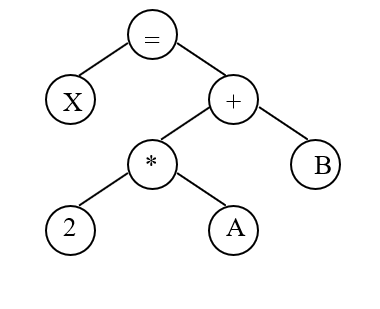
\includegraphics[width=0.5\paperwidth]{C:/Users/Admin/Desktop/Github/question_bank/LyX/static/img/9597-HCI-2019-P2-Q7}
\par\end{center}

This tree can then be read using the following algorithm:

process left subtree 

process right subtree 

read root node

This will give \texttt{X 2 A {*} B + =} which is the reverse Polish
form of the expression.
\begin{enumerate}
\item Using diagrams to help the explanation, or otherwise, show how a computer
can use a stack to evaluate the expression from its reverse Polish
form. \hfill{}{[}4{]}
\item The tree in the example could be stored in an array called TREE.
\noindent \begin{center}
\begin{tabular}{|c|c|c|c|}
\hline 
TREE{[}9{]} &  &  & \tabularnewline
\hline 
TREE{[}8{]} &  & -1 & \tabularnewline
\hline 
TREE{[}7{]} &  & 5 & \tabularnewline
\hline 
TREE{[}6{]} &  &  & \tabularnewline
\hline 
TREE{[}5{]} & 2 &  & \tabularnewline
\hline 
TREE{[}4{]} &  &  & \tabularnewline
\hline 
TREE{[}3{]} & X &  & \tabularnewline
\hline 
TREE{[}2{]} &  &  & \tabularnewline
\hline 
TREE{[}1{]} & B &  & \tabularnewline
\hline 
TREE{[}0{]} & = & 3 & 4\tabularnewline
\hline 
\end{tabular}
\par\end{center}

The values in each location in the array are: node value; left pointer;
right pointer. Where no left or right pointer exists the rouge value
-1 is used. Copy and complete the array for the example. (Note that,
since in the example there are only seven nodes, three rows of the
array will be unused.) \hfill{}{[}5{]}
\item Draw a tree similar to the one in the example which would represent
the expression:
\begin{center}
\texttt{Y = 2 {*} (A + B) \textendash{} (A \textasciicircum{} 2)} 
\par\end{center}

where \texttt{x \textasciicircum{} y} means $\mathtt{x^{y}}$.\hfill{}{[}3{]}
\item Using the algorithm in the example, and your tree, write out the reverse
Polish form of the expression in \textbf{part} (c). \hfill{}{[}3{]}
\end{enumerate}
{[}SPLIT\_HERE{]}
\item \textbf{{[}HCI/PRELIM/9597/2019/P2/Q8{]} }

Using the following numbers as an example, show how the numbers can
be sorted in ascending order using a \textbf{quick sort}. For each
pass, show the numbers swapped and the sub lists after splitting. 
\noindent \begin{center}
435, 646, 344, 54, 23, 98
\par\end{center}

\noindent \begin{flushleft}
\hfill{}{[}7{]}
\par\end{flushleft}

{[}SPLIT\_HERE{]}
\end{enumerate}
 
\end{document}
